Dans ce chapitre, nous décrivons la mise en œuvre des analyses statiques
précédentes. Nous commençons par décrire la représentation intermédiaire
utilisée: Newspeak. La chaîne de compilation est explicitée, partant de C pour
aller jusqu'à Tyspeak, sur lequel nous décrivons d'un algorithme d'inférence de
types à la Hindley-Milner, reposant sur l'unification et le partage de
références. Toutes ces étapes sont implantées dans le langage
OCaml~\link{ocaml}.

En réalité, Newspeak (et donc Tyspeak) utilise une représentation de plus bas
niveau que \langname donc les règles sont légèrement différentes.

% TODO mieux décrire les 3

\section{Newspeak}
\label{sec:npk}

Newspeak est un langage intermédiaire conçu pour être un bon support d'analyses
statiques, contrairement à des langages conçus pour les programmeurs comme C.
Plusieurs points en font un langage pratique à utiliser. Tout d'abord, il est
suffisamment expressif pour compiler tout C, y compris de nombreuses extensions
GNU utilisées dans le noyau Linux (section~\label{sec:gnuc}), et des traducteurs
automatiques depuis C et Ada existent (section~\label{sec:compil}).

Ensuite, ses instructions sont orthogonales et minimales: il existe en général
une seule manière de faire les choses. Par exemple, le flot de contrôle est
restreint à la boucle infinie et au saut en avant («\emph{break}» généralisé).

Enfin, lorsque certaines constructions sont ambigües, un choix est fait. Par
exemple, l'évaluation des arguments d'une fonction est faite de manière
explicite, les tailles des types sont indiqués à chaque déclaration de variable,
etc. Sa sémantique d'exécution (ainsi qu'une partie des étapes de compilation
depuis C) est décrites dans \cite{newspeak}. Sa syntaxe est donnée dans la
figure~\ref{fig:stx-npk}.

\begin{figure}

\def\npkstyle#1{\mathrm{#1}}

\begin{align*}
\gramdef{Instruction}{s}
    {\npkstyle{Set} (lv, e, st}{Affectation}
    {\npkstyle{Copy} (lv, lv, n)}{Copie}
    {\npkstyle{Guard} (e)}{Garde}
    {\npkstyle{Decl} (var, t, blk)}{Déclaration}
    {\npkstyle{Select} (blk, blk)}{Branchement}
    {\npkstyle{InfLoop} (blk)}{Boucle infinie}
    {\npkstyle{DoWith} (blk, x)}{Nommage de bloc}
    {\npkstyle{Goto} (x)}{Saut}
    {\npkstyle{Call} ([(e_i, t_i)], f, [(lv_i, t_i)])}
            {Appel de fonction}
    {END}
\\ \\
\gramdef{Bloc}{blk}
    {[i_i]}{Liste d'instructions}
    {END}
\\ \\
\gramdef{Left-value}{lv}
    {\npkstyle{Local} (x)}{Locale}
    {\npkstyle{Global} (x)}{Globale}
    {\npkstyle{Deref} (e, n)}{Déréférencement}
    {\npkstyle{Shift} (lv, e)}{Décalage}
    {END}
\\ \\
\gramdef{Expression}{e}
    { \npkstyle{CInt} (n) }{Entier}
    { \npkstyle{CFloat} (d)}{Flottant}
    { \npkstyle{Nil} }{ Pointeur nul }
    { \npkstyle{Lval} (lv, t)}{Accès mémoire}
    { \npkstyle{AddrOf} (lv) }{Adresse de variable}
    { \npkstyle{AddrOfFun} (x, [t_i], [t_i])}{Adresse de fonction}
    { \npkstyle{UnOp} (unop, e) }{Opérateur unaire}
    { \npkstyle{BinOp} (binop, e_1, e_2) }{Opérateur binaire}
    {END}
\\ \\
\gramdef{Fonction}{f}
    { \npkstyle{FunId} (x)}{Appel par nom}
    { \npkstyle{FunDeref} (e)}{Appel par pointeur}
    {END}
\\ \\
\gramdef{Type}{t}
    { \npkstyle{Scalar} (st) }{Type scalaire}
    { \npkstyle{Array} (t, n)}{Tableau}
    { \npkstyle{Region} ([(n_i, t_i)], n')}{Structure/union}
    {END}
\\ \\
\gramdef{Type scalaire}{st}
    { \npkstyle{Int} (n) }{Entier}
    { \npkstyle{Float} (n) }{Flottant}
    { \npkstyle{Ptr} }{ Pointeur sur données}
    { \npkstyle{FunPtr}}{ Pointeur sur fonction}
    {END}
\end{align*}
\caption{Syntaxe simplifiée de Newspeak}
\label{fig:stx-npk}
\end{figure}

\section{Chaîne de compilation}
\label{sec:compil}

\begin{figure}
  \centering
  \begin{tikzpicture}\shorthandoff{!}
\tikzstyle{file}=[draw, shape=rectangle, node distance=2.2cm, minimum
height=1cm, shade, top color=white,
    bottom color=blue!50!black!20, draw=blue!40!black!60, very thick];

\node [file] (c1) {\textcolor{black}{.c}};
\node [file, below of=c1] (c2) {\textcolor{black}{.c}};
\node [node distance=2.2cm, below of=c2] (c3) {};

\node [file, minimum height=0, node distance=5mm, above of=c3,draw] (c3b) {.adb};
\node [file, minimum height=0, node distance=5mm, below of=c3,draw] (c3s) {.ads};

\path (c3b.north west) ++(-3mm,3mm) [draw,dotted] rectangle ($(c3s.south east)+(3mm,-3mm)$);

\node [below of=c3, node distance=2.2cm] (c4){};

\node [file, right of=c1] (cc1) {\textcolor{black}{.c}};
\node [file, right of=c2] (cc2) {\textcolor{black}{.c}};
\node [node distance=2.2cm, right of=c3] (cc3) {};

\node [below of=cc3, node distance=2.2cm](cc4){};

\draw[->] (c1) -- node[above] {{\tiny \ttfamily gcc -E}} (cc1);
\draw[->] (c2) -- (cc2);

\node [file, right of=cc1] (no1) {\textcolor{black}{.no}};
\node [file, right of=cc2] (no2) {\textcolor{black}{.no}};
\node [file, right of=cc3] (no3) {\textcolor{black}{.no}};

\node [below of=no3, node distance=2.2cm](no4){};

\draw[->] (cc1) -- node[above] {{\tiny \ttfamily c2newspeak -c}} (no1);
\draw[->] (cc2) --  (no2);

\draw[->] ($ (c3b.north east)!0.5!(c3s.south east) + (3mm,0) $) -- node[above] {\tiny \ttfamily ada2newspeak -c} (no3);


\node [file, right of=no2] (npk) {\textcolor{black}{.npk}};

\node [right of=no3, node distance=2.2cm](npk2){};
\node [right of=no4, node distance=2.2cm](npk3){};

\node[draw, ellipse, right of=no2, minimum height=3cm]{};

\draw[->] (no1) -- node {} (npk);
\draw[->] (no2) -- node[above] {{\tiny \ttfamily c2newspeak}} (npk);
\draw[->] (no3) -- node {} (npk);


\node [file, right of=npk](warn) {\textcolor{black}{.warn}};

\node [right of=npk3, node distance=3cm](analyser2){};

\draw[->] (npk) -- node[above] {{\tiny \ttfamily penjili}} (warn);

\draw[->] (c4)   -- node[above, text depth=3pt] {\footnotesize Pr\'etraitement} (cc4);
\draw[->] (cc4)  -- node[above, text depth=3pt] {\footnotesize Compilation} (no4);
\draw[->] (no4)  -- node[above, text depth=3pt] {\footnotesize \'Edition de liens} (npk3);
\draw[->] (npk3) -- node[above, text depth=3pt] {\footnotesize Analyse} (analyser2);
\end{tikzpicture}

  \caption{Compilation depuis Newspeak}
\label{fig:compil-npk}
\end{figure}

%TODO Mettre à jour la figure

La compilation vers C est faite en trois étapes (figure~\ref{fig:compil-npk}):
prétraitement du code source, compilation de C prétraité vers \newspeak{}, puis
compilation de \newspeak{} vers ce langage.

La première étape consiste à prétraiter les fichiers C source avec le logiciel
\texttt{cpp}, comme pour une compilation normale. Cette étape interprète les
directives comme \texttt{\#include}, \texttt{\#ifdef}, À cet étape, les
commentaires sont aussi supprimés.

Une fois cette passe effectuée, le résultats est un ensemble de fichiers C
prétraités, c'est-à-dire des unités de compilation.

Puisque la directive \texttt{\#include} est textuelle, ces fichiers sont très
grands et donnent lieu à beaucoup de duplication dans les passes suivantes.

Sur cette représentation (du C prétraité), il est possible d'ajouter des
annotations de la forme \texttt{/*!npk [...] */} qui pourront être accessible
dans l'arbre de syntaxe abstrait des passes suivantes.

À ce niveau, les fichiers sont passés à l'outil \texttt{c2newspeak} qui les
traduit vers Newspeak. Comme il sera décrit dans la section~\ref{sec:gnuc}, la
plupart des extensions GNU C sont acceptés en plus du C ANSI. Dans cette étape,
les types et les noms sont résolus, et le programme est annoté de manière à
rendre les prochaines étapes indépendante du contexte. Par exemple, chaque
déclaration de variable est adjointe d'une description complète du type.

Lors de cette étape, le flôt de contrôle est également simplifié. C en effet
propose de nombreuses constructions ambigües ou redondantes.

Au contraire, Newspeak propose un nombre réduit de constructions. Rappelons que
le but de ce langage est de faciliter l'analyse statique: des constructions
orthogonales permettent donc d'éviter la duplication de règles sémantique, ou de
code lors de l'implémentation d'un analyseur.

Par exemple, plutôt que de fournir une boucle \emph{while}, une boucle
\emph{do/while} et une boucle for, Newspeak fournit une unique boucle
\npkWhile{}. La sortie de boucle est compilée vers un \npkGoto{}\cite{goto}, qui
est toujours un saut vers l'avant (similaire à un «\emph{break}» généralisé).

Newspeak est conçu pour l'analyse statique par interprétation abstraite. Il a
donc une vue de bas niveau sur les programmes. Par exemple, aucune distinction
n'est faite entre l'accès à un champ et l'accès à un l'élément d'un tableau
(tous deux sont traduits par un décalage numérique depuis le début de la zone
mémoire). Pour supprimer cette ambiguïté, il faut s'interfacer dans les
structures internes de \texttt{c2newspeak}, où les informations nécessaires sont
encore présentes.

Ensuite, les différents fichiers sont liés ensemble. Cette étape consiste
principalement à s'assurer que les hypothèses faites par les différentes unités
de compilation sont cohérentes entre elles. Les objets marqués \texttt{static},
invisibles à l'extérieur de leur unité de compilation, sont renommés afin qu'ils
aient un nom unique.

Enfin, l'implantation d'un algorithme d'inférence pour les systèmes de types
décrits dans les chapitres~\ref{cha:typbase} et~\ref{cha:qualifs} est assez
simple. Puisqu'ils sont suffisament proches du lambda calcul simplement typé, on
peut utiliser une variante de l'algorithme W de Damas et
Milner~\cite{DamasMilner}. On utilise l'optimisation classique qui consiste à se
reposer sur le partage de références pour réaliser l'unification, plutôt que de
faire des substitutions explicites. Puisque ces systèmes de types sont
monomorphes, on présente une erreur si des variable de type libres sont
présentes.

À la fin de cette étape, on obtient soit un programme complètement annoté, soit
une erreur de type.

\begin{figure} % fig:exunif:c {{{

  \insertcode{ex-unif-c.c}

  \caption{Exemple de programme C à compiler}
\label{fig:exunif:c}
\end{figure} % }}}

Prenons l'exemple de la figure~\ref{fig:exunif:c} et typons-le «à la main». On
commence par oublier toutes les étiquettes de type présentes dans le programme.
Celui-ci devient alors:

\insertcode{exunif-code.c}

La premiere ligne introduit deux variables. On peut noter leurs types respectifs
(inconnus pour le moment) $t_1$ et $t_2$. La première affectation \texttt{p =
\&x} implique que les deux côtés du signe «$=$» ont le même type. À gauche, le
type est $t_2$, et à droite $Ptr(t_1)$. On applique le même raisonnement à la
seconde affectation: à gauche, le type est $t_1$ et à droite \texttt{Int}. On en
déduit que le type de x est \texttt{Int} et celui de p est \verb!Ptr(Int)!.

\insertcode{lambda-types.ml}

% TODO c'est le code d'un typeur naif

Pour implanter cet algorithme, on représente les types de données du programmes
à typer par une valeur de type \texttt{ml\_type}. En plus des constantes de
types comme int ou float, et des constructeurs de type comme pair et fun, le
constructeur Var permet d'exprimer les variables de types (inconnues ou non).

Celles-ci sont numérotées par un int, on suppose avoir à disposition deux
fonctions manipulant un compteur global d'inconnues.

\insertcode{exunif-counter.ml}

De plus, un module gère les environnements de typage. Il peut être implanté avec
des listes d'association ou des tables de hachage, par exemple. Sa signature
est:

\insertcode{exunif-env.ml}

Reprenons l'exemple précédent. Partant d'un environnement vide (Env.empty), on
commence par l'étendre de deux variables. Comme on n'a aucune information, il
fait allouer des nouveaux noms d'inconnues (qui correspondent à $t_1$ et $t_2$):

\insertcode{exunif-1.ml}

La première instruction indique que les deux côtés de l'affectation doivent
avoir le même type.

\insertcode{exunif-2.ml}

\begin{figure}
  \centering
  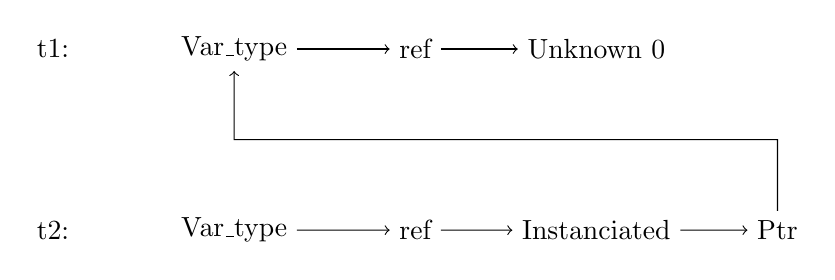
\begin{tikzpicture}
    [scale=2.3]

    \node at (0,  0) (n0a) {t1:};
    \node at (0, -1) (n0b) {t2:};

    \node at (1,  0) (n1a) {Var\_type};
    \node at (2,  0) (n2a) {ref};
    \node at (3,  0) (n3a) {Unknown 0};

    \node at (1, -1) (n1b) {Var\_type};
    \node at (2, -1) (n2b) {ref};
    \node at (3, -1) (n3b) {Instanciated};
    \node at (4, -1) (n4b) {Ptr};

    \draw [->] (n1a) -- (n2a);
    \draw [->] (n2a) -- (n3a);

    \draw [->] (n1b) -- (n2b);
    \draw [->] (n2b) -- (n3b);
    \draw [->] (n3b) -- (n4b);

    \draw [->] (n4b) -- ++ (0, 0.5) -| (n1a);

  \end{tikzpicture}
  \caption{Partage lors de l'unification}
\label{fig:unifsharing}
\end{figure}

Ici il se passe plusieurs choses intéréssantes. D'une part nous faisont appel à
une fonction externe typeof qui retourne le type d'une expression sous un
environnement (dans une implantation complète il s'agirait d'un appel récursif).
Dans ce cas, \texttt{typeof lhs1 env} est identique à \texttt{Env.get lhs1 env}
et \texttt{typeof rhs1 env} à \texttt{Ptr\_type t1}. L'autre aspect intéressant
est la dernière ligne: la fonction \texttt{unify} va modifier en place les
représentations des types afin de les rendre égales. L'implantation de
\texttt{unify} sera décrite plus tard. Dans ce cas précis, elle va faire pointer
la référence dans t2 vers t1 (figure~\ref{fig:unifsharing}).

Enfin, la seconde affectation se déroule à peu près de la même manière.

\insertcode{exunif-3.ml}

Ici \texttt{typeof lhs2 env} est identique à
\verb!Ptr_type (Env.get "p" env)! et \texttt{typeof lhs2 env} à \texttt{Const\_type Int\_type}. Et dans cas,
l'unification doit se faire entre t1 et \texttt{Const\_type Int\_type}: cela
mute la référence derrière t1 (figure~\ref{fig:typeunifref}).

\begin{figure}
  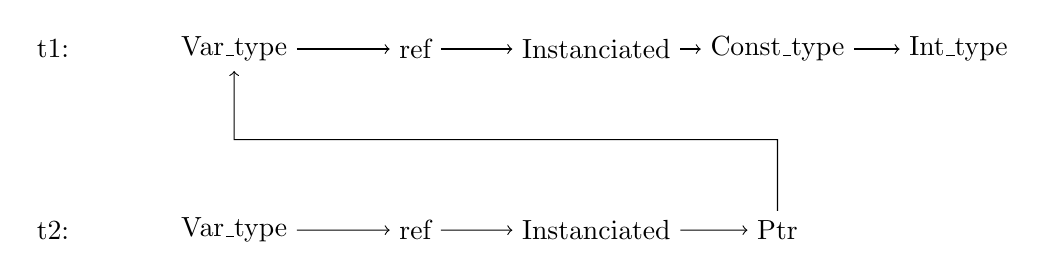
\begin{tikzpicture}
    [scale=2.3]

    \node at (0,  0) (n0a) {t1:};
    \node at (0, -1) (n0b) {t2:};

    \node at (1,  0) (n1a) {Var\_type};
    \node at (2,  0) (n2a) {ref};
    \node at (3,  0) (n3a) {Instanciated};
    \node at (4,  0) (n4a) {Const\_type};
    \node at (5,  0) (n5a) {Int\_type};

    \node at (1, -1) (n1b) {Var\_type};
    \node at (2, -1) (n2b) {ref};
    \node at (3, -1) (n3b) {Instanciated};
    \node at (4, -1) (n4b) {Ptr};

    \draw [->] (n1a) -- (n2a);
    \draw [->] (n2a) -- (n3a);
    \draw [->] (n3a) -- (n4a);
    \draw [->] (n4a) -- (n5a);

    \draw [->] (n1b) -- (n2b);
    \draw [->] (n2b) -- (n3b);
    \draw [->] (n3b) -- (n4b);

    \draw [->] (n4b) -- ++ (0, 0.5) -| (n1a);

  \end{tikzpicture}
  \caption{Unification par mutation de références}
\label{fig:typeunifref}
\end{figure}

L'essence de l'algorithme d'inférence se situe donc dans 2 fonctions. D'une
part, \texttt{unify} qui réalise l'unification des types grâce à au partage des
références. D'autre part, la \texttt{typeof} qui encode les règles de typage
elles-mêmes et les applique à l'aide de \texttt{unify}.

\subsection*{Algorithme d'unification}

Voici une implantation de la fonction \texttt{unify}.

Celle-ci prend en entrée deux types $t_1$ et $t_2$. À l'issue de l'exécution de
\texttt{unify}, ces deux types doivent pouvoir être considérés comme égaux. Si
ce n'est pas possible, une erreur sera levée.

La première étape est de réduire ces deux types, c'est-à-dire à transformer les
constructions \texttt{Var (ref (Instanciated t))} en \texttt{t}.

Ensuite, cela dépend des formes qu'ont les types réduits:

\begin{figure}
  \centering
  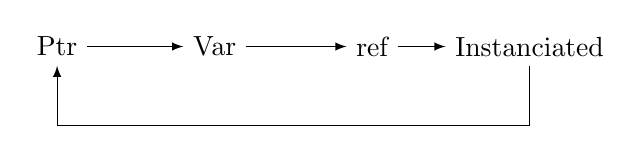
\begin{tikzpicture}
    [every node/.style={node distance=2cm}
    ,>=latex
    ]

    \node (n1) {Ptr};
    \node[right of=n1] (n2) {Var};
    \node[right of=n2] (n3) {ref};
    \node[right of=n3] (n4) {Instanciated};

    \draw [->] (n1) -- (n2);
    \draw [->] (n2) -- (n3);
    \draw [->] (n3) -- (n4);

    \draw [->] (n4) -- ++ (0, -1cm) -| (n1);

  \end{tikzpicture}
  \caption{Cycle dans le graphe de types}
\label{fig:typecycle}
\end{figure}

\begin{itemize}

\item si les deux types sont inconnus (de la forme \texttt{Var (ref
(Instanciated t))}), on fait pointer l'une des deux références vers le premier
type. Notons que cela crée un type de la forme \texttt{Var (ref (Instanciated
(Var (ref (Unknown n)))))} qui sera réduit lors d'une prochaine étape
d'unification.

\item si un type est inconnu et pas l'autre, il faut de la même manière affecter la
référence. Mais en faisant ça inconditionnellement, cela peut poser problème:
par exemple en tentant d'unifier \texttt{a} avec \verb!Ptr(a)! on pourrait
créer un cycle dans le graphe (figure~\ref{fig:typecycle}).
Pour éviter cette situation, il suffit de s'assurer que le type inconnu n'est
pas présent dans le type à affecter.

\item si les deux types sont des types de base (comme $\tInt$ ou $\tFloat$)
égaux, on ne fait rien.

\item si les deux types sont des constructeurs de type, il faut que les
constructeurs soient égaux. On unifie en outre leurs arguments deux à deux.

\item si les deux types sont des types structure, on étudie les types de leurs
champs. On commence par unifier les types des champs de même nom, et on
on ajoute à l'un les champs exclusifs à l'autre.

\item dans les autres cas, l'algorithme échoue.

\end{itemize}

\section{Architecture de \ptrtype}
\label{sec:ptrtype-archi}

L'outil \ptrtype{} lit un programme Newspeak (ou un fichier C), et réalise
l'inférence de qualificateurs. En sortie, il affiche soit le programme
complètement annoté, soit une erreur. Le cœur de l'outil est dans la

Si l'argument à \ptrtype{} est un fichier C, il est tout d'abord compilé vers
Newspeak grâce à l'utilitaire \texttt{c2newspeak}. Ensuite, les autres passes
travaillent sur une représentation intermédiaire proche de Newspeak, mais où des
étiquettes de type supplémentaires sont ajoutées. Ce type de représentation
intermédiaire (polymorphe en le type des étiquettes) est \texttt{'a Tyspeak.t}.

\begin{figure}
\insertcode{implem-process.ml}
\caption{Fonction principale de \ptrtype{}}
\label{fig:implem-process}
\end{figure}

Le reste de l'outil est résumé dans la fonction
\texttt{process\_npk} (figure~\ref{fig:implem-process}):

\begin{itemize}

\item Grâce à la fonction \verb!convert_unit : Newspeak.t -> unit Tyspeak.t!,
  on ajoute des étiquettes «vides» (toutes égales à \verb!() : unit!).

\item L'ensemble des fonctions du programme est trié topologiquement selon la
  relation~$\preceq$ définie par $f \preceq g \eqdef \textrm{«} g
  \textrm{ apparaît dans la définition de } f \textrm{»}$. Cela est fait en
  construisant une représentation de $\preceq$ sous forme de graphe, puis en
  faisant un parcours en largeur de celui-ci.

% TODO et pour les fonctions mutuellement récursives?

\item Les annotations extérieures sont alors lues (variable \texttt{exttbl}), ce
  qui permet de créer un environnement initial.

\item Les types de chaque fonction sont inférés, par le biais de la fonction
  suivante:

\begin{Verbatim}
val infer : Newspeak.fid list
         -> Types.simple Env.t
         -> 'a Tyspeak.t
         -> Types.simple Tyspeak.t
\end{Verbatim}

\item Le programme obtenu, de type \texttt{Types.simple Tyspeak.t}, est affiché
  sur le terminal.

\end{itemize}

\section{Inférence de types}

L'inférence de types consiste à remplacer les étiquettes de type \texttt{unit}
par des étiquettes de type \texttt{simple} (autrement dit de vraies
représentations de types).

Cette étape se fait de manière impérative: on peut créer de nouveaux types avec
\texttt{new\_unknown} et unifier deux types
avec \texttt{unify}. Leurs types sont:

\begin{verbatim}
val new_unknown : unit -> Types.simple
val unify : Types.simple -> Types.simple -> unit
\end{verbatim}

La fonction \texttt{infer} s'appuie sur un ensemble de fonctions récursivement
définies portant sur chaque type de fragment: \texttt{infer\_fdec} pour les
déclarations de fonction, \texttt{infer\_exp} pour les expressions,
\texttt{infer\_stmtkind} pour les instructions, etc.

Les règles de typage sont implantées par \texttt{new\_unknown} et
\texttt{unify}. Par exemple, pour typer une déclaration
(figure~\ref{fig:implem-unif-stmt}), on crée un nouveau
type \texttt{t0}. On étend l'environnement courant avec cette nouvelle
association et sous ce nouvel environnement, on type le bloc de portée de la
déclaration.

\begin{figure}[h] %{{{

\insertcode{infer-unif-stmt.ml}

\caption{Inférence des déclarations de variable et appels de
         fonction}

\label{fig:implem-unif-stmt}
\end{figure}%}}}

De même, pour typer un appel de fonction, on infère le type de ses arguments et
left-values de retour. On obtient également le type de la fonction (à partir du
type de la fonction présent dans l'environnement, ou du type du pointeur de
fonction qui est déréférencé), et on unifie ces deux informations.

On peut donner quelques exemples, comme:

\begin{itemize}
  \item addition de deux flottants (dans \texttt{infer\_binop}):

\begin{verbatim}
let infer_binop op (_, a) (_, b) =
  match op with
    (* [...] *)
    | N.PlusF _ ->
        unify a Float;
        unify b Float;
        Float
\end{verbatim}

  \item adresse d'une left-value (dans \texttt{lval\_type}):

\begin{verbatim}
| T.AddrOf lv ->
    let lv' = infer_lv env lv in
    let ty = lval_type env lv in
    (T.AddrOf lv', Ptr (Kernel, ty))
\end{verbatim}

  \item déréférencement d'une left-value (dans \texttt{lval\_type}):

\begin{verbatim}
| T.Deref(e, _sz) ->
    let (_, te) = infer_exp env e in
    let t = new_unknown () in
    unify (Ptr (Kernel, t)) te;
    t
\end{verbatim}

\end{itemize}

\section{Unification}

\begin{figure}
\insertcode{implem-types.ml}
\caption{Représentation des types}
\label{fig:implem-typ}
\end{figure}

Les types de données utilisés sont donnés dans la figure~\ref{fig:implem-typ}.
Les types \langname{} sont représentés soit par un constructeur de type
«résolu» immutable comme \texttt{Int}, soit par une référence dans le cas
d'une variable inconnue (placée alors derrière le constructeur \texttt{Var}).

Ces références contiennent une valeur du type
\texttt{simple var\_type}\footnote{
  Ce type est polymorphe pour pouvoir être repris dans l'unification des
  qualificateurs (figure~\ref{fig:implem-qualifs}).
}, c'est-à-dire:

\begin{itemize}
\item soit un numéro d'inconnue (constructeur \texttt{Unknown})\footnote{On
  place le numéro dans un enregistrement pour abstraire l'entier sous-jacent, en
  empêchant par exemple de faire de l'arithmétique sur celui-ci.}.

\item soit un type résolu (constructeur \texttt{Instanciated}) si cette
  inconnue a été unifiée avec un type concret.
\end{itemize}

Ce système peut créer des représentations de types arbitrairement longues, comme
par exemple:

\texttt{Var (ref (Instanciated (Var (ref (Instanciated Int)))))}

Cela est dû au fait que \texttt{fun x -> Var (ref (Instanciated x))} est typée
\texttt{simple -> simple} et peut donc être appliquée à loisir. Pour éviter cet
effet d'allongement, on définit une fonction \texttt{shorten} qui supprime ces
chaînes (figure~\ref{fig:implem-shorten}).

\begin{figure}

  \insertcode{implem-shorten.ml}

\caption{Fonction de racourcissement des représentations de types}
\label{fig:implem-shorten}
\end{figure}

La fonction d'unification, quant à elle, commence par raccourcir ses deux
arguments puis faire une analyse de cas par filtrage.

Les cas principaux pour unifier deux types réduits \texttt{sta} et \texttt{stb}
sont:

\begin{itemize}

\item \texttt{sta} et \texttt{stb} sont deux inconnues. Alors on modifie l'un
  pour pointer sur l'autre. Les références étant uniques et partagées, cela
  revient à substituer l'un par l'autre dans toutes les représentations de
  types.

\item Un type est concret, l'autre une inconnue. Dans ce cas on modifie le
  second comme étant un \texttt{Instanciated} du premier. Il faut vérifier que
  le type inconnu remplacé n'apparaît pas dans le type concret, sinon on créé un
  cycle. Ce cas a lieu par exemple quand on cherche à unifier $t$ avec
  $\ptrK{t}$. Il faut alors signaler une erreur, ce que fait la fonction
  \texttt{occurs\_check\_failed}.

\item Les deux types sont des types concrets. Alors ils sont de la forme
  respective
  $C (t_1, …, t_n)$
  et
  $D (u_1, …, u_m)$ où $C$ et $D$ sont des constructeurs de type avec
  respectivement $n$ et $m$ arguments\footnote{
    Le cas $n = 0$ ou $m = 0$ correspond aux types concrets comme $\tInt$ ou
    $\tFloat$.
  }. Si $C = D$ et
  $n = m$, alors on unifie récursivement chaque $t_i$ avec $u_i$. Sinon on lève
  une erreur (fonction \texttt{type\_clash}).

\end{itemize}

Cette analyse de cas est implantée dans la fonction \texttt{unify_now}
(figure~\ref{fig:implem-unify-now}).

\begin{figure}
  \insertcode{implem-unify.ml}
\caption{Fonction d'unification}
\label{fig:implem-unify-now}
\end{figure}

Pour les pointeurs, il est nécessaire de définir des fonctions similaires sur
les qualificateurs (figure~\ref{fig:implem-qualifs}).

\begin{figure}

  \insertcode{implem-qualifs.ml}

  \caption{Qualificateurs}
\label{fig:implem-qualifs}

\end{figure}

\begin{figure}

\insertcode{unify-main.ml}

\caption{Unification directe ou retardée}
\label{fig:implem-lazy}
\end{figure}

La fonction appellée directement par le reste du code, appellée \texttt{unify},
peut retarder l'unification (figure~\ref{fig:implem-lazy}). Dans ce cas, la
paire de types à unifier est mise dans une liste d'attente qui sera unifiée
après le parcours du programme. Le but est d'instrumenter l'inférence de types
afin de pouvoir en faire une exécution «pas à pas».

\section{Exemple}

Lançons l'analyse sur un petit exemple:

\begin{verbatim}
int f(int *x) { return (*x + 1); }
\end{verbatim}

L'exécution de notre analyseur affiche un programme complètement annoté:

\begin{verbatim}
 % ptrtype example.c
f : (Ptr (Int)) -> (Int)
Int (example.c:1#4)^f(Ptr (Int) x) {
  (.c:3#4)^!return =(int32)
    (coerce[-2147483648,2147483647]
      ( ( ([(x_Ptr (Int) : Ptr (Int))]32_Int
            : Int
          )
          + (1 : Int)
        ) : Int
      ) : Int
    );
}
\end{verbatim}

L'opérateur \texttt{coerce[a,b]} est un artefact de Newspeak, destiné à détecter
les débordements d'entiers lors d'une analyse de valeurs par interprétation
abstraite. Dans le cas de notre analyse, les valeurs ne sont pas pertinentes et
cet opérateur peut être vu que comme un «plus» unaire typé $(\tInt) → \tInt$.

Un exemple de cas d'erreur sera décrit dans la section~\ref{sec:demo-unif}.

% TODO pas de conclusion

% TODO trop de figures

% vim: spelllang=fr
